\documentclass[11pt]{article}

\usepackage{loblib}


\usepackage{amssymb,amsfonts,units,multicol,empheq,centernot}
\usepackage{algorithmicx,algpseudocode,verbatim,comment}
\usepackage{tikz,tikzrput}

\usepackage{geometry}
\usepackage{url}
\usepackage{lipsum}


\usetikzlibrary{arrows}
\usetikzlibrary{calc}



\usepackage{adforn}
\pdfmapfile{+ OrnementsADF.map}

\newcommand{\info}{
\vspace{.55cm}
\name \texttt{(\netid)}

\today \\
}



%%%%%%%%%%%%%%%%%%%%%%%%%%%%%%%%%%%%%%%%%%%%%%%%%

\renewcommand{\coursename}{ Algorithms  }
\renewcommand{\coursenumber}{ CS 4820 }
\renewcommand{\name}{ Bryce Evans  }
\renewcommand{\netid}{bae43}
\renewcommand{\today}{September 12, 2013}
\renewcommand{\hwnum}{1}
\renewcommand{\hwtitle}{NP-Completeness }


%%%%%%%%%%%%%%%%%%%%%%%%%%%%%%%%%%%%%%%%%%%%%%%%%

\usepackage{fancyhdr}
\pagestyle{fancy}
\fancyhead[L]{\lobclaw{simple}\vspace{-1.5mm}\coursenumber HW\hwnum: \textit{\hwtitle}}
\fancyhead[R]{\name - \netid}


\title{\coursename}
\author{\name}
\date{\today}

\begin{document}


\lobtitle
\info

\lobwatermark

\section{Near Cliques}

\subsection{Solution}

Prove: \textit{Clique Problem} $\leq_p$ \textit{Near Clique Problem}\\

The Clique of Size $k$ Problem in NP-Complete reduces to the Near Clique of Size $k$ Problem. Both the near clique and full clique problems take inputs $G = (V,E)$, and output \texttt{True} if a subgraph  $g$ (defined separately in each problem) has the property $g \subseteq G$, and \texttt{False} otherwise. Create the efficient reduction $\sigma$ as follows: \\



\textbf{$\sigma$ Reduction:}
Given graph $G = (V,E)$, add two nodes $v_1, v_2$ that connect to every $v \in V$. Solving the near clique problem on this graph solves the clique problem as well.\\

If a clique of size $k$ exists in $G$, then adding $v_1, v_2$ and
connecting them to every other vertex will form a near clique of size
$k+2$ because no edge connects $v_1$ and $v_2$. If one or more edges
are missing, then adding additional nodes that are not connected to
each other will cause at least 2 edges to now be missing among the
nodes, and therefore the near clique algorithm will return
false. \lobtomb

\pagebreak
\textbf{Example:}
\begin{center}

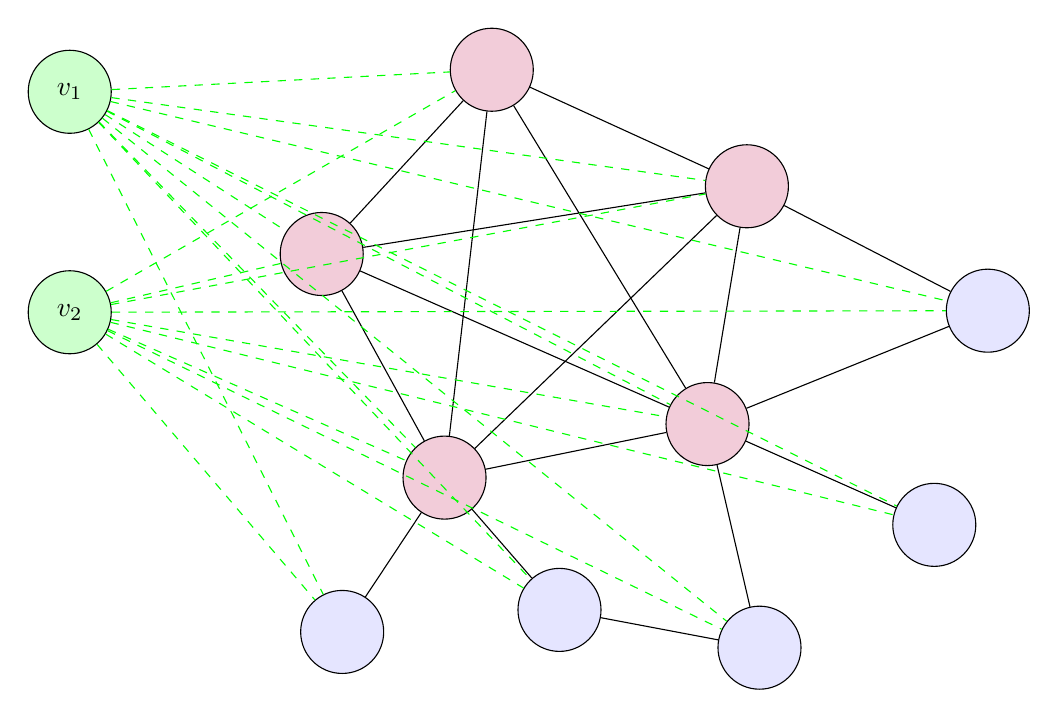
\begin{tikzpicture}
[>=stealth',scale=.2,auto=center,every node/.style={circle,fill=blue!10,minimum size=3em,draw}]

\node[fill=purple!20] (a) at (21.8,-8.6) {};
\node[fill=purple!20] (b) at (38,-16) {};
\node[fill=purple!20] (c) at (35.5,-31.1) {};
\node[fill=purple!20] (d) at (18.8,-34.5) {};
\node[fill=purple!20] (e) at (11,-20.3) {};

\node (f) at (53.3,-23.9) {};
\node (g) at (49.9,-37.5) {};
\node (h) at (26.1,-42.9) {};
\node (i) at (38.8,-45.3) {};
\node (j) at ((12.3,-44.3) {};

\node[fill=green!20] (v1) at (-5,-10) {$v_1$};
\node[fill=green!20] (v2) at (-5,-24) {$v_2$};

%clique
\foreach \from/\to in {a/b,a/c,a/d,a/e,b/c,b/d,b/e,c/d,c/e,d/e}
\draw (\from) edge(\to);

\foreach \from/\to in {b/f,c/f,c/g,i/h,d/h,c/i,d/j}
\draw (\from) edge(\to);

\foreach \to in {a,b,c,d,e,f,g,h,i,j}
\draw [green] (v1) edge [dashed] (\to);

\foreach \to in {a,b,c,d,e,f,g,h,i,j}
\draw [green] (v2) edge [dashed] (\to);

\end{tikzpicture}\\



Graph $G$ with clique $k_5$ highlighted in red and $v_1,v_2$ connected to every vertex in $G$. A near clique of size $k+2$ forms between the red and green colored nodes.
\end{center}

\textbf{Runtime of $\sigma$}
\begin{align*}
&\text{Add nodes $v_1,v_2$: } &O(1)\\ 
&\text{Connect $v_1,v_2$ to $v\, \forall v \in V$: } &O(V)\\ 
&\textbf{Total Reduction Runtime: } &O(V)\\
\end{align*}

\textbf{$\tau$ Reduction:}
Construct a function $\tau$ that takes the output of $\sigma$ and converts it to a valid solution of the clique problem:\\

The construction of $\tau$ is trivial - the output of $\sigma$ is equivalent to the clique problem. A near clique of size $k+2$ will exist after adding $v_1,v_2$ if and only if a clique of size $k$ existed in $G$ prior.  \\

\textbf{Runtime of $\tau$ }
\begin{align*}
&\text{Output boolean is equivalent to solution to clique problem: } &O(1)\\ 
&\textbf{Total Reduction Runtime: } &O(1)\\
\end{align*}


\subsection{Efficient Verifier:}
Given a solution set $S$ of $k$ elements to the near clique problem, remove $v_1,v_2$ and corresponding edges. Take this graph and verify that each node has an edge to every other node. If every node connects to all others, the algorithm should have returned \texttt{True}, and if not, then \texttt{False}. \\

\textbf{Runtime of Verifier }
\begin{align*}
&\text{Remove $v_1,v_2$}&O(1)\\
&\text{Verify all $k$ nodes connect to others} &O(k^2)\\ 
&\textbf{Total Runtime: } &O(k^2)\\
\end{align*}

\lobsectionbreak

\section{Submatrix Domination}
\lobwatermark

\subsection{Solution}

Prove: \textit{Clique Problem} $\leq_p$ \textit{Near Clique Problem}\\

The Clique of Size $k$ Problem in NP-Complete reduces to the Matrix Subdomination Problem. The  clique problem takes input $G = (V,E)$, and output \texttt{True} if there exists a clique of size $k$ that exists in $G$ and \texttt{False} otherwise. Create the efficient reduction $\sigma$ as follows: \\

\textbf{$\sigma$ Reduction:}
Given Graph $G$, find if it contains a clique of size $k$. Create adjacency matrices $M_k, M_G$ for both the clique and $G$, such that each row and column $(r_i,c_i)$ represents some node $i \in G$. If $i$ is connected to $j \in G$, $M_G[i,j],M_G[j,i] = 1$. The main diagonal has all values of $2$.  \\

Permute the columns so that the taken columns are consecutive. This is an isomorphism to the original graph as this essentially just a renaming of the nodes. Because the graph is undirected, the matrix is symmetric and the rows are then consecutive like the columns.\\


Because of the properties of this adjacency matrix, diagonals are the highest values in the matrices because no other value can be $>1$, meaning diagonals cannot be dominated by anything but another value in the diagonal. This forces no node to be accidentally paired up with another node by domination. For all diagonal values of $M_k$ to be dominated in $M_G$, the diagonals must align to each other, as no value in $M_G$ other than a diagonal is $\geq 2$. \\


Because of the properties of adjacency matrices, if every value in the matrix is a 1 (excluding diagonal), then every node in that set is connected to all others in the set. Therefore, the mapping of $r(\cdot),c(\cdot)$ returns the set of nodes that form the clique. If $M_G$ contains $M_k$, then $G$ contains the clique and the algorithm returns \texttt{True}. It is guaranteed that if such a submatrix is found that it is a clique because the matrix must be centered on the diagonal, with each node the columns represent being connected to each other. If the submatrix is found within $M_G$ then, the clique exists within $G$. \lobtomb  \lobwatermark 



\pagebreak
\textbf{Example:} Find if graph $G$ contains $k_3$ (in red).\\
\begin{center}
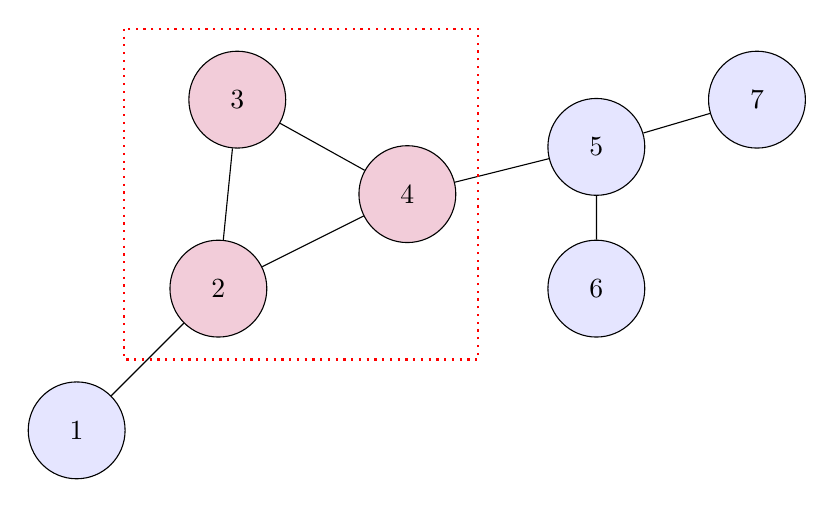
\begin{tikzpicture}
[>=stealth',scale=1.2,auto=center,every node/.style={circle,fill=blue!10,minimum size=3.5em,draw}]

\node (a) at (.5,.5) {1};
\node[fill=purple!20] (b) at (2,2) {2};
\node[fill=purple!20] (c) at (2.2,4) {3};
\node[fill=purple!20] (d) at (4,3) {4};
\node (e) at (6,3.5) {5};
\node (f) at (6,2) {6};
\node (g) at (7.7,4) {7};


\foreach \from/\to in {a/b,b/c,b/d,c/d,d/e,e/g,e/f}
\draw (\from) edge(\to);

\draw[red,thick,dotted] (1,4.75)  rectangle (4.75,1.25);

\end{tikzpicture}\\



Graph $G$ with clique $k_3$ highlighted.
\end{center}

In this simple example, the nodes are numbered in way such that the clique is formed by consecutively numbered nodes, causing the submatrix to be easily spotted in $M_G$. Note that this is not always the case, but the vertices may be renumbered to cause this.\\
 
\[M_k = 
\left[ {\begin{array}{*{3}c}
   2 & 1 & 1  \\
   1 & 2 & 1 \\
   1 & 1 & 2  \\
 \end{array} } \right]
\quad
 M_G = 
\left[ {\begin{array}{*{7}c}
   2 & 1 & 0 & 0 & 0 & 0 & 0  \\
   1 & \textcolor{red} 2 & \textcolor{red}1 & \textcolor{red}1 & 0 & 0 & 0  \\
   0 & \textcolor{red}1 & \textcolor{red}2 & \textcolor{red}1 & 0 & 0 & 0  \\
   0 & \textcolor{red}1 & \textcolor{red}1 & \textcolor{red}2 & 1 & 0 & 0  \\
   0 & 0 & 0 & 1 & 2 & 1 & 1  \\
   0 & 0 & 0 & 0 & 1 & 2 & 0  \\
   0 & 0 & 0 & 0 & 1 & 0 & 2  \\
 \end{array} } \right]
\]\\


\textbf{Runtime of $\sigma$}
\begin{align*}
&\text{Compute $M_k$: } &O(k^2)\\ 
&\text{Compute $M_G$: } &O(V^2)\\ 
&\textbf{Total Reduction Runtime: } &O(V^2)\\
\end{align*}


\textbf{$\tau$ Reduction:}
Construct a function $\tau$ that takes the output of $\sigma$ and converts it to a valid solution of the clique problem:\\

This is a decision problem with only a boolean output. \texttt{True} and \texttt{False} map to the same values and the reduction is trivial.\\

\textbf{Runtime of $\tau$ }
\begin{align*}
&\text{Output boolean is equivalent to solution of vertex cover: } &O(1)\\ 
&\textbf{Total Reduction Runtime: } &O(1)\\
\end{align*}


\subsection{Efficient Verifier:}
Given a solution set $S$ to the submatrix domination problem, test all values of $A$ into $r(\cdot),c(\cdot)$. If every value of $r(\cdot),c(\cdot)$ matches, then the algorithm should have returned \texttt{True}, and if not, then \texttt{False}. \\

\textbf{Runtime of Verifier }
\begin{align*}
&\text{Iterate through $m_1$ rows and $n_1$ columns of $A$:} &O(n_1m_1)\\
&\textbf{Total Runtime: } &O(n_1m_1)\\
\end{align*}

\lobsectionbreak

\section{Party Invitations}

\subsection{Solution}

\lobwatermark

Prove: \textit{Vertex Cover} $\leq_p$ \textit{Party Invitation Problem}\\

The Vertex Cover Problem in NP complete reduces to the party invitation problem. If we can solve the party invitation problem, we could solve the vertex cover problem as well. Create this efficient reduction $\sigma$ as follows:  \\

The party invitation takes inputs:
\begin{itemize}
\item a set of lists $L = \{l_1,l_2,l_3, \ldots, l_{k}\}$
\item a set of corresponding values $M = \{m_1, m_2, m_3, \ldots, m_k\}$ of the \textit{minimum} number of elements that can be chosen from $l_i \in L$.
\item $n$ - the max number of elements that can be chosen from all lists
\end{itemize}

The solution to the problem outputs a boolean \texttt{True} if there exists a set of elements smaller than $n$ in cardinality  that satisfies all the constraints, and \texttt{False} otherwise.\\

Recall that vertex cover has given $G = (V,E)$, and $k$, the max number of vertices that can be chosen in the cover, with the constraint $\forall e = (u,v) \in E$, $e$ is connected to some $o \in O$. Vertex cover returns a boolean \texttt{True} if there exists some set of vertices $S$ such that $|S| \leq k $ and \texttt{False} otherwise. \\

\textbf{$\sigma$ Reduction:}
Consider $n$ to be the number of edges, $|E|$. For all $e \in E$, at least 1 vertex must be taken, so $M = \{1,1,1,\ldots, 1\}$. For all $e = (u,v) \in E$, construct a list $L' = \{\{u_1,v_1\},\{u_2,v_2\},\{u_3,v_3\},\ldots, \{u_k,v_k\}\}$ Use $L'$ as the input set of lists for the party invitation problem. This reduction maintains all of the constraints for Vertex Cover -  each edge $e$ must have one valid vertex be chosen to cover it where a valid vertex is one that has $e$ as an endpoint. \\

\textbf{Runtime of $\sigma$}
\begin{align*}
&\text{Calculate number of edges: } &O(E)\\ 
&\text{Create List $L'$: } &O(E)\\ 
&\text{Find $M$: } &O(1)\\
&\textbf{Total Reduction Runtime: } &O(E)\\
\end{align*}

\textbf{$\tau$ Reduction:}
Construct a function $\tau$ that takes the output of $\sigma$ and converts it to a valid solution of the vertex cover problem:\\

The construction of $\tau$ is trivial - the output of $\sigma$ is equivalent to if a vertex cover of size $k$ exists. Vertex Cover $(VC)$  will return true if and only if the party invitation problem $(PI)$ returns true because each edge $e \in G$ requires at least one vertex it is connected to to be chosen. This is maintained in $PI$ because each set has a minimum number of elements needed to be picked to be 1, with valid elements being only vertices touching that edge. Therefore, under the constraints of $PI$, each edge will have at least one vertex that it is connected to be chosen. \lobtomb \\

\textbf{Runtime of $\tau$ }
\begin{align*}
&\text{Output boolean is equivalent to solution of vertex cover: } &O(1)\\ 
&\textbf{Total Reduction Runtime: } &O(1)\\
\end{align*}


\subsection{Efficient Verifier:}
Given a solution set $S$ of $n$ elements to $PI$, a polynomial verifier is as follows:\\

For each element $e$ in list $l \in L$, check every element in $S$ and see if it exists. If every $e$ exists in $S$, the algorithm should have returned \texttt{True}, and if not, then \texttt{False}. \\

\textbf{Runtime of Verifier }
\begin{align*}
&\text{Iterate through every $e$ in list $l \in L$,}\\
&\text{$\quad$ with $m$ being the total number of these elements: $m = \sum_{l \in L} |l|$} &O(m)\\ 
&\text{Iterate through every element of $S$ } &O(n)\\ 
&\textbf{Total Runtime: } &O(nm)\\
\end{align*}

\lobsectionbreak

\vspace*{2.7cm}
\hspace*{7cm} 
\lob[lobblue, scale=1.5]{83} \hfill
\vspace*{-.7cm}

\end{document}